\documentclass[a4paper]{article}

%% Language and font encodings
\usepackage[english]{babel}
\usepackage[utf8x]{inputenc}
\usepackage[T1]{fontenc}

%% Sets page size and margins
\usepackage[a4paper,top=3cm,bottom=2cm,left=3cm,right=3cm,marginparwidth=1.75cm]{geometry}

%% Useful packages
\usepackage{amsmath}
\usepackage{amsfonts}
\usepackage{graphicx}
\usepackage[colorinlistoftodos]{todonotes}
\usepackage[colorlinks=true, allcolors=blue]{hyperref}
\usepackage{subfig}
\usepackage{xcolor}

\newcommand{\aw}[1]{{\color{blue} [AW: #1]}}
\newcommand{\jm}[1]{{\color{red} [JM: #1]}}
\newcommand{\ap}[1]{{\color{red} [AP: #1]}}

\title{Non-Periodic Edge States \footnote{ \aw{I prefer ``Edge States in Disordered Media''. The edge states may be periodic; the point is that we are studying such states in a medium (material) which is not. The term ``disordered'' is appropriate: it is not just that the pattern of the medium doesn't repeat itself, the material actually has no order: seeing what the material looks like in one place doesn't tell you very much about what it looks like in another because the atomic positions and onsite potentials are random. In, for example, a ``quasi-crystal'' the structure of the medium is ordered in the sense that it can be generated by a deterministic algorithm. This is not true for the media we are considering.} } }
\author{Jonathan Michala and Alexander Pierson}

\begin{document}

\aw{some things I want to make a note of:} 
\begin{itemize}
\item We have to make the bibliography: I can show you how to do this (it's a pain) using BibDesk
\item Deadline for report is December 17th (the last day of finals)
\item A couple of things which need to be worked out at some point (I think after we submit the writeup):
\begin{itemize}
\item In addition to mapping out the ``local index'' at each point, we should map out the size of the ``local gap'': the size of the smallest eigenvalue of the matrix $B$. This should give us a sense of when the edge states will actually be stable.
\item When we consider disorder of the atom positions, we should replace $t \rightarrow t e^{1 - r/r_0}$ where $r$ is the distance between atoms and $r_0$ is the distance between atoms *without disorder* and do the same for complex hopping too.
\item We should also consider the effect of the localization parameter
\end{itemize}
\end{itemize}
\aw{Nature of final report from Duke math website:} \\

Nature of Final Product \\

The final product for your research independent study will be a formal paper (as opposed to an informal report) that meets the criteria listed below. \\

1. The paper describes important aspects of the work done during the course. \\

2. The paper is thoughtful, well organized, and well written. It should be carefully proofread. \\

3. The paper communicates well to as broad an audience as would reasonably be assumed to have interest in your research topic. \\

4. The first part of the paper (two pages minimum) describes the broader context in which the project took place. This section should be written in a way that is understandable to an individual who has no specialized knowledge beyond the standard course content regularly offered by the Duke math department. \\

Specialized technical terms should be defined or avoided. \\

If your project involved a particular problem in a field of pure mathematics, it should be related to broader questions within that field. \\

If your project involved an application of mathematics, appropriate background material should be explained to motivate the problem and set it in a suitable context. \\

If non-standard mathematical techniques are used, they should be compared to standard techniques. \\

The final paper may, at the discretion of the instructor, include relevant excerpts from any paper or report that you had written for a previous related independent study course or in connection with a previous related research project. However, such excerpts may only constitute a small portion of your final paper. \\

Work on the final paper, especially on that part that explains the broader context of the research, may be begun early in the semester. \\

Student will e-mail an electronic copy of their final paper to the Director of Undergraduate Studies of mathematics on or before the last day of final exams. \\

\newpage

\maketitle

\section{Background}
\aw{This you should be able to mostly lift from the Summer project. The main points are (1) controlling wave propagation is of significant interest for a range of applications: acoustics, electromagnetics, quantum mechanics... (2) particular interest in ways of controlling waves which are robust against imperfections in the medium/device (3) in ``topological insulators'' it is observed that waves which propagate at the edge of such media (edge states) are highly robust against perturbations, related with topological invariants associated with the bulk Hamiltonian (Chern number) (4) The aim of this project is to investigate to what extent this story (topological invariants and robust edge states) generalizes when the medium is strongly disordered i.e. we make a perturbation such that the medium is no longer periodic at all because of onsite potentials which vary significantly across the material and varying atomic positions. Good to contrast with the summer when we considered robustness of edge states to strong perturbations on the edge. Here we are studying perturbations of the \emph{whole medium}. Note also that we are considering a case where the usual topological invariant doesn't seem to be relevant at all since the medium is not periodic. This is where the Loring index comes in: it is an index which agrees with the Chern number when the medium is periodic, but since it is not defined through Bloch states it is well defined when the medium is not periodic (aperiodic) as well.}
\section{Loring Index} \aw{Note on title: let's call it the Bott index as in 2009HastingsLoring} \\

\aw{I would start with e.g. ``We start by introducing the Bott index abstractly, we discuss its relevance in physics below. (new paragraph) It is well known that a set of $n$ Hermitian matrices which commute may be simultaneously diagonalized, i.e.... Given a set of $n$ Hermitian matrices which \emph{almost} commute, i.e....''} \\

\aw{We can then talk about physics below ``The Bott index can be used to define a local topological index in a disordered medium as follows...'' } \\

\aw{Another thing (I apologize for being a little loose when I have talked about this in our meetings): our audience for this report is mathematicians. So let's not talk about ``eigenstates'' until we are talking about physics. At that point we should mention ``it is common in quantum mechanics to refer to eigenvectors of self-adjoint operators as eigenstates''} \\

Let $\Psi$ be a state in two dimensions with entries $\Psi_{m,n}$, where $m$ describes location with respect to one dimension (whether that be an $x$-coordinate in $\mathbb{R}^2$ or a cell index along an edge) and where $n$ describes location with respect to the other dimension.
Define $X$ and $Y$ to be an operators that act on a state $\Psi$ in the following way:
$$(X \Psi)_{m,n} = m\Psi_{m,n}, \quad (Y \Psi)_{m,n} = n\Psi_{m,n}.$$
Eigenstates of these operators are localized in their corresponding dimensions.
Therefore, when looking for localized eigenstates of a system whose Hamiltonian is $H$, our aim is to find simultaneous eigenstates of all three operators $H$, $X$, and $Y$.\\
This is not always possible, however.
Suppose $A_1,...,A_n$ are Hermitian matrices that all commute with each other.
Then, they can be simultaneously diagonalized, i.e. $U^* A_i U$ is diagonal for all $i \in \{1,...,n\}$ for some unitary matrix $U$.
So if $H$, $X$, and $Y$ commute, we can find simultaneous eigenstates of them.
Now, suppose $A_1,...,A_n$ do not all commute, but their commutators are bounded:
$$[A_i,A_j] \leq \delta \quad \forall\; i,j \in \{1,...,n\}$$
for some $\delta$.
If $n = 2$, there must exist some $\widetilde{A}_1, \widetilde{A}_2$ which commute and satisfy:
$$||\widetilde{A}_1 - A_1||, ||\widetilde{A}_2 - A_2|| \leq \epsilon(\delta)$$
where $\epsilon(\delta) \rightarrow 0$ as $\delta \rightarrow 0$ and where $||M||$ denotes the largest eigenvalue of $M$.\\
But if $n = 3$, there may or may not exist $\widetilde{A}_1, \widetilde{A}_2, \widetilde{A}_3$ such that they all commute with each other and satisfy:
$$||\widetilde{A}_i - A_i|| \leq \epsilon(\delta), \quad \i \in \{1,2,3\}.$$
This existence holds if and only if
$$\frac{1}{2}\; \text{sig} \begin{pmatrix}
A_3 & A_1 + iA_2\\
A_1 - iA_2 & - A_3
\end{pmatrix} = 0$$
where sig$(M)$ is the signature, or number of positive eigenvalues minus negative eigenvalues, of $M$. This is known as the Bott Index of three matrices, denoted Bott($A_1,A_2,A_3$).
Thus, to calculate the index at a particular location, $\lambda_1,\lambda_2$ in our system near an eigenvalue $\lambda_3$ of $H$ \jm{Is this the correct motivation?} we look at
$$\text{Bott}(X-\lambda_1,Y - \lambda_2, H - \lambda_3) = \frac{1}{2}\; \text{sig}\begin{pmatrix}
H - \lambda_3 & (X - \lambda_1) + i(Y - \lambda_2)\\
(X - \lambda_1) - i(Y - \lambda_2) & - (H - \lambda_3)
\end{pmatrix}.$$
If this matrix has an eigenvalue less than a specified norm $\epsilon$, we say that the triple $(\lambda_1,\lambda_2,\lambda_3)$ is in the joint pseudo-spectrum of the given lattice.\aw{it is $(\lambda_1,\lambda_2,\lambda_3)$ that is in the joint pseudo-spectrum: the pseudo-spectrum is a generalization of the spectrum (the set of eigenvalues), and the joint pseudo-spectrum is a generalization of the joint spectrum}
If a triple is not in the pseudo-spectrum, we then compute the Bott index using the above calculation. \aw{Hastings-Loring explains the Loring index a little. The point is that } \\\\
To compute the signature of $B$ efficiently, we use the $LDL^T$ decomposition of $B$.
$D$ is a block diagonal matrix with blocks of either size $1 \times 1$ or $2 \times 2$.
Let $a$ and $b$ be the number of positive and negative $1 \times 1$ blocks in $D$, respectively.
By J.R. Bunch, L. Kaufman (Need ref), the signature of $B$ is equivalent to the signature of $D$ which is $a - b$. \aw{we should identify why $L D L^T$ works, e.g. ``it is known (see ref...) that the signature of $B$ equals the signature of the diagaonal matrix $D$ which appears in $L D L^T$ factorization''}

\section{Loring Index in Haldane Model}

\aw{Good idea to have this section. We should motivate what we do here, e.g. ``We now show numerically that the Bott index is equal to the Chern number where both are defined (i.e. when the medium is periodic so that the eigenstates of the Hamiltonian are Bloch states)'' }	\\

\aw{We should mention the issue with boundary conditions and having to shift the $X$ and $Y$ operators}

In the Haldane Model, $m$ and $n$ are the indices of cells on a hexagonal, atomic lattice, where each cell has two sites, labeled $A$ and $B$.
Thus we define our $X$ and $Y$ operators as follows:
$$X_{i,i} = \left\lfloor \frac{i-1}{2} \right\rfloor \;\text{mod}\;m, \quad\quad Y_{i,i} = \left\lfloor \frac{i-1}{2m} \right\rfloor$$
with $X_{i,j} = Y_{i,j} = 0$ for $i \neq j$. 
We compute the pseudo-spectrum and Bott index on the Haldane model lattice with complex hopping and see that in the topological case, the Bott index behave much like the Chern number:
on a lattice with edges, the index is $+1$ on the interior and transitions to 0 across the edge;
on a periodic lattice, the index is $+1$ everywhere.
In the trivial case we see a Bott index of 0 everywhere on edged and periodic lattices, which is analogous to the Chern number.
This is shown in Figure \ref{fig:Bott Haldane}.
\begin{figure}
\centering
\subfloat{{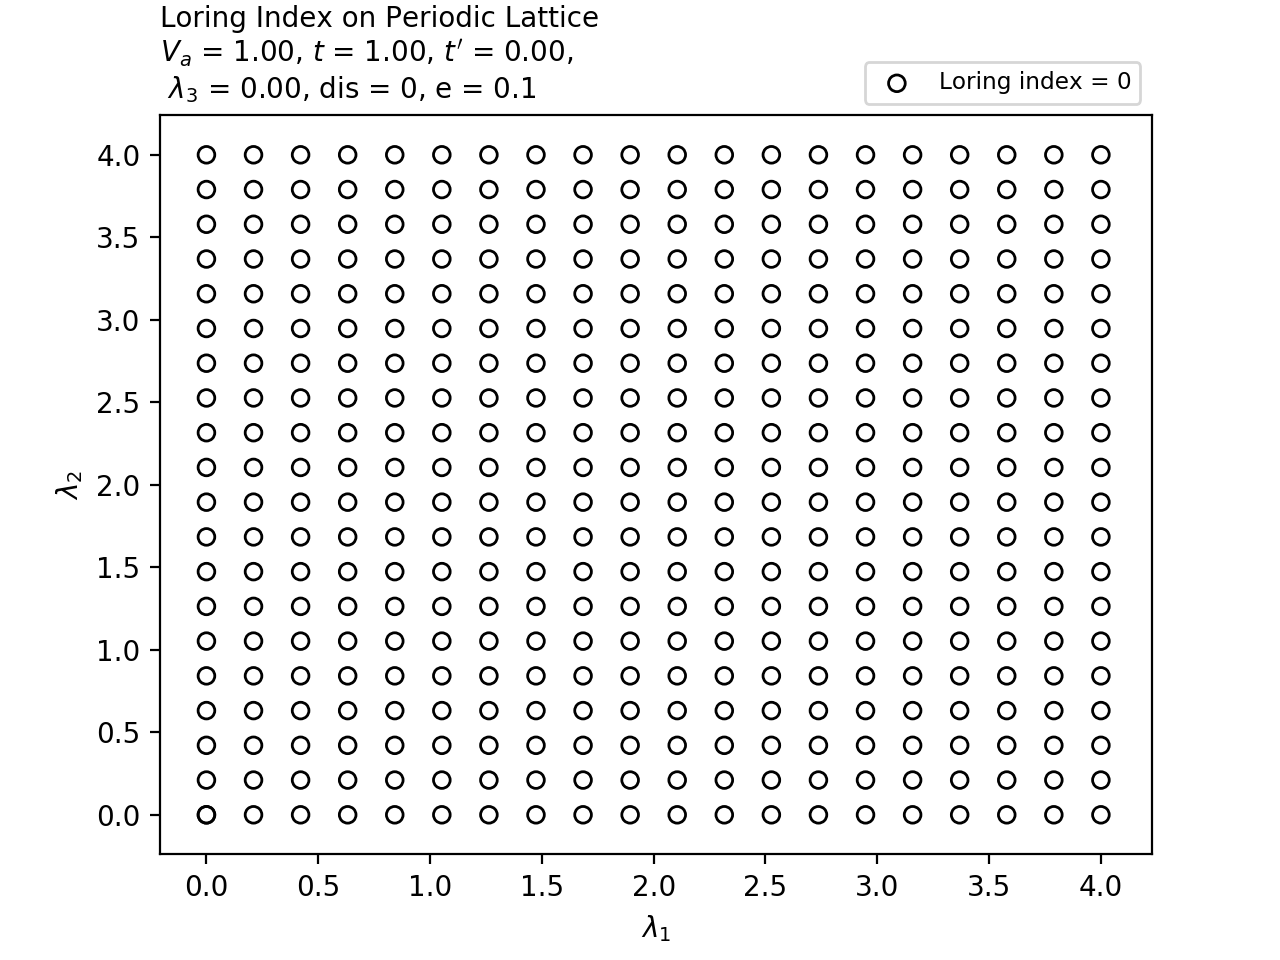
\includegraphics[width=.45\linewidth]{figures/periodic_triv} }}%
\subfloat{{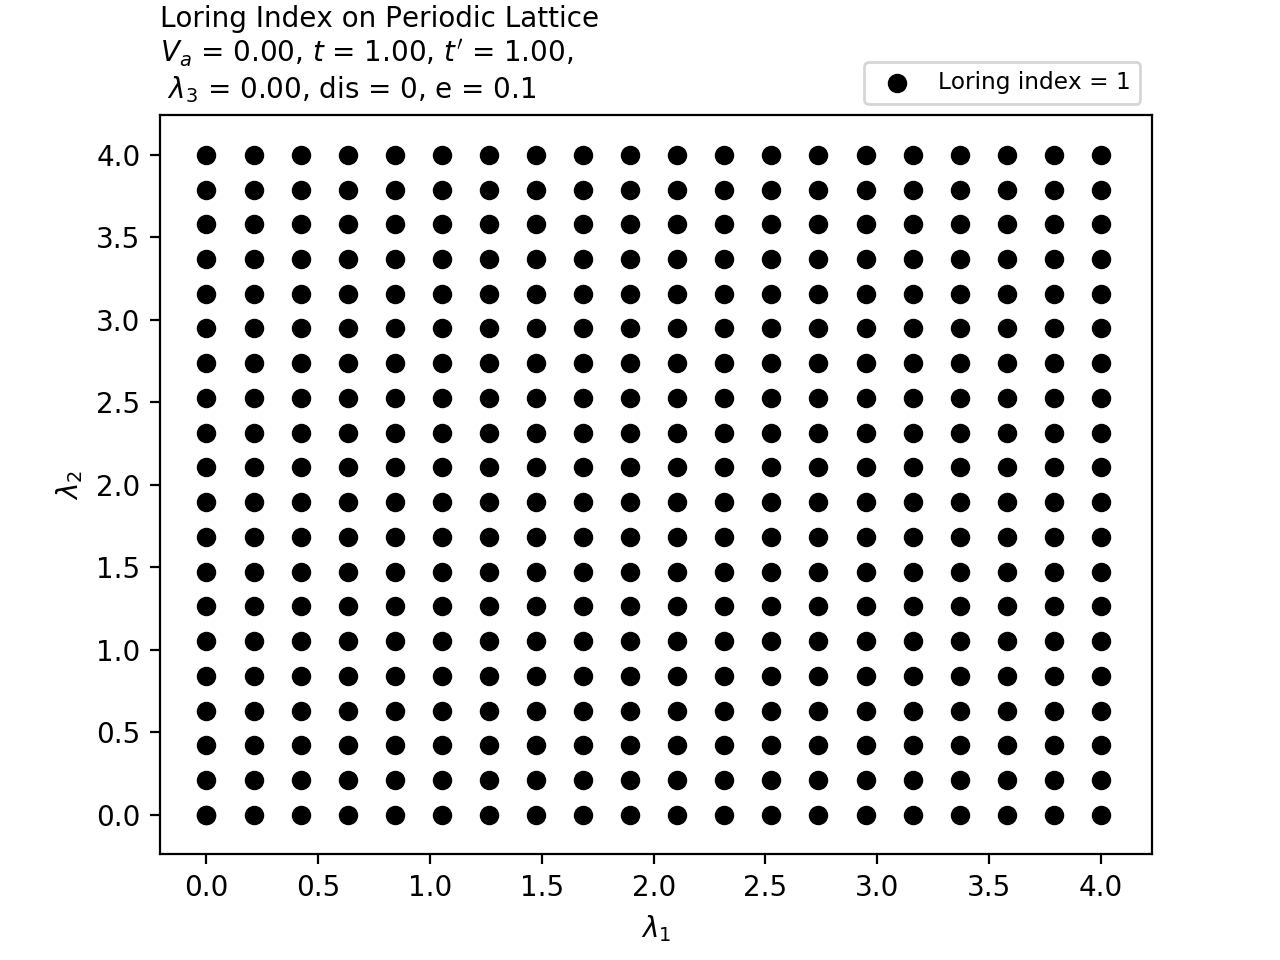
\includegraphics[width=.45\linewidth]{figures/periodic_top} }}%

\subfloat{{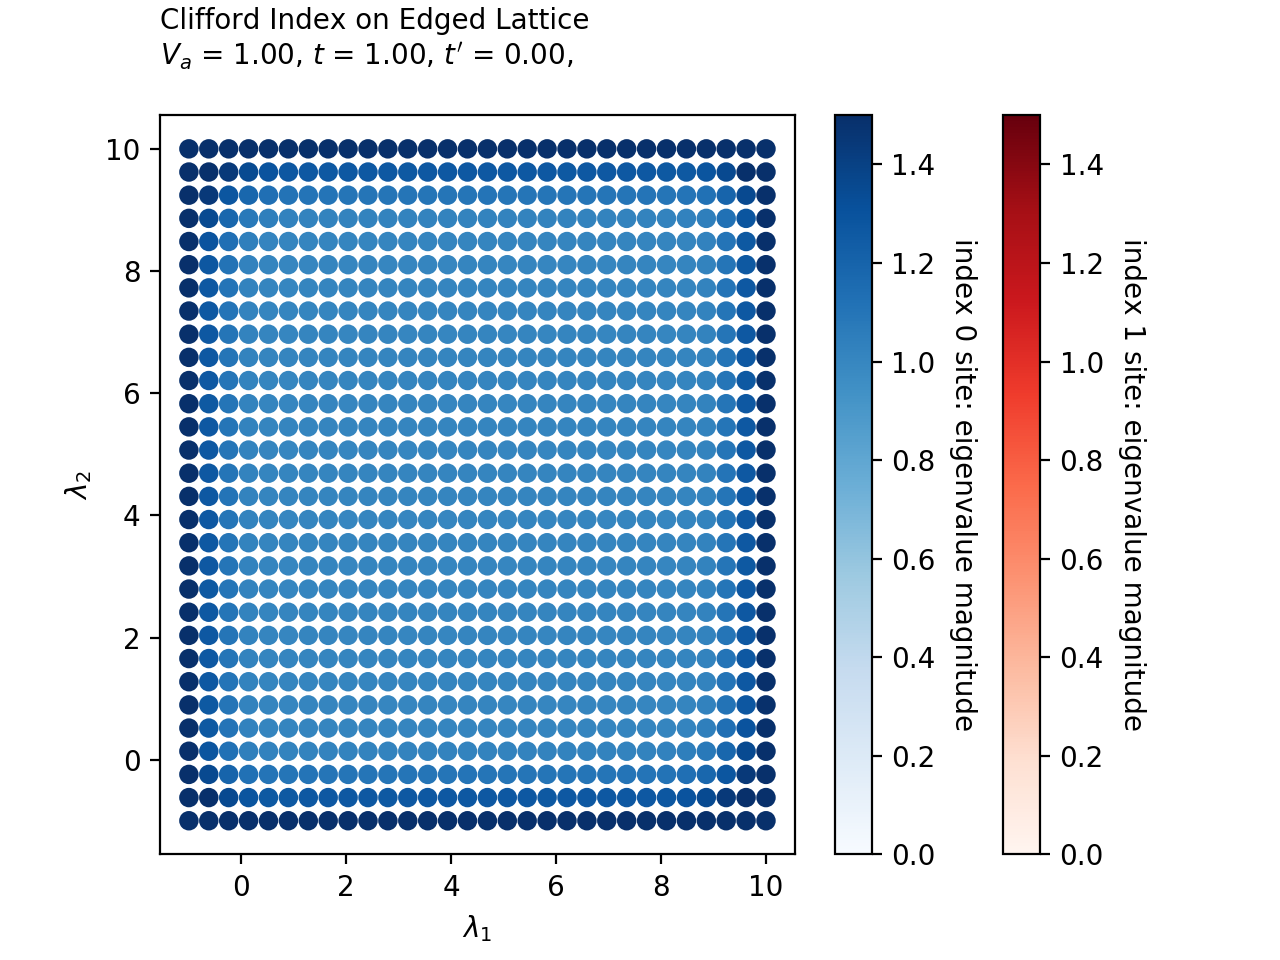
\includegraphics[width =.45\linewidth]{figures/edged_triv} }}%
\subfloat{{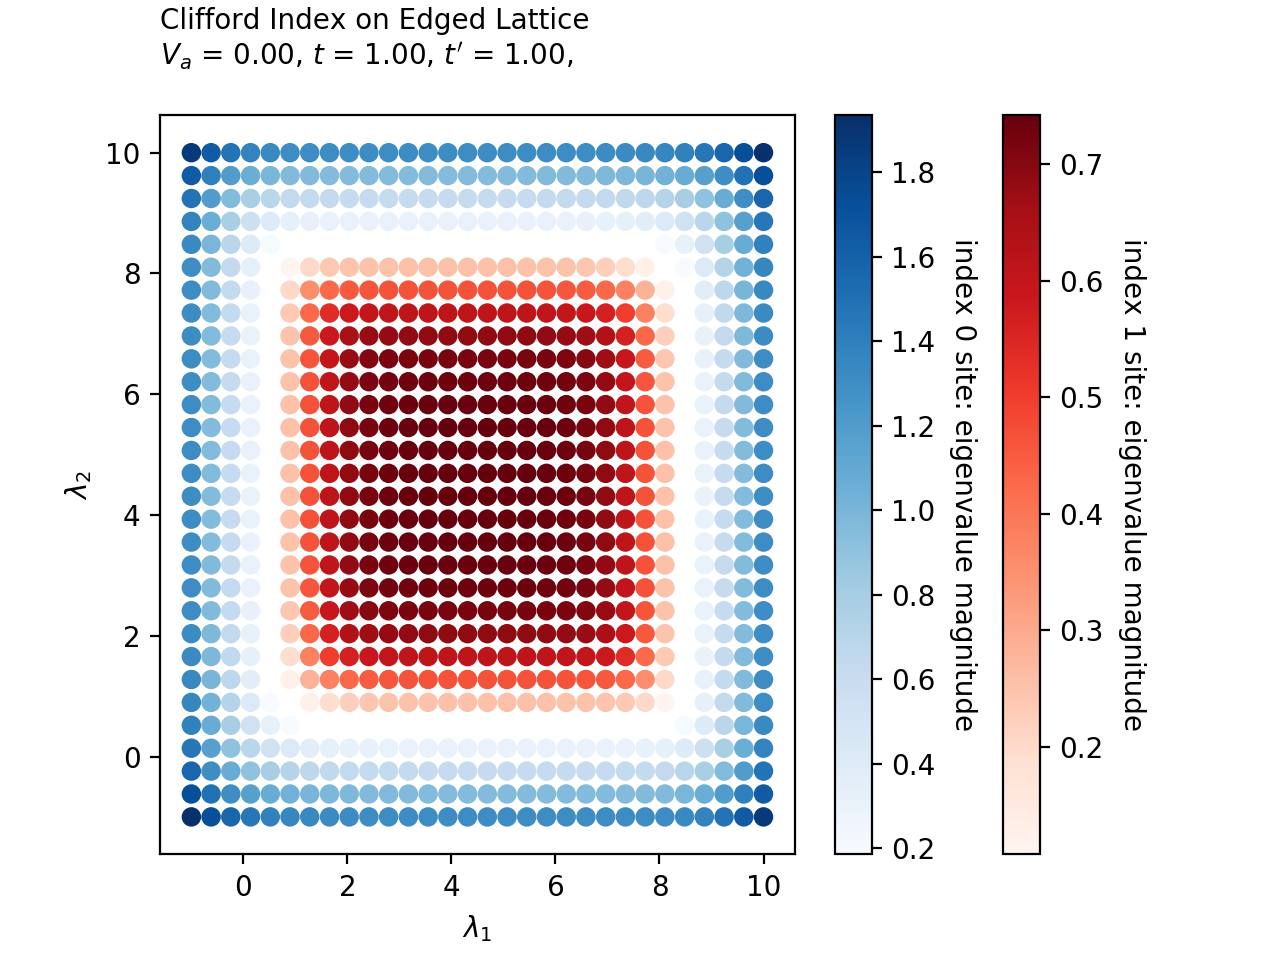
\includegraphics[width =.45\linewidth]{figures/edged_top} }}%
\caption{The top left is a trivial, periodic lattice; the top right is a topological, periodic lattice; the bottom left is a trivial, edged lattice; and the bottom right is a topological, edged lattice.
Each site in these figures represents a $(\lambda_1,\lambda_2,\lambda_3)$ triple with $\lambda_3 = 0$.
If a site is red, then it is in the pseudo-spectrum, i.e. $B(X - \lambda_1, Y - \lambda_2, H - \lambda_3)$ has a near-zero eigenvalue.
If a site is not in the pseudo-spectrum, then it is colored black for Bott index 1 and white for Bott index 0, where the Bott index is defined as one half the signature of $B$. \aw{very nice figure. It is a little funny that the corners for the Haldane model don't all look the same. I don't quite understand why this would be.} \\
}%
\label{fig:Bott Haldane}%
\end{figure}
The advantage of the Bott index compared to the Chern number is that the Chern number can only be defined on a periodic structure, whereas the Bott index can be computed on non-periodic media.
We will use this advantage to study the robustness of waves on non-periodic media.

\section{Propagation in Haldane Model}
As expected, we find that localized waves propagate along the boundary of the edged, topological lattice since this is a boundary between Bott index 0 and Bott index 1. Figures to come.

\aw{Clarify that this shows that the Bott index and Chern number predict edge states similarly}

\section{\texorpdfstring{$p_x + ip_y$}{px + ipy} Model}
\aw{We should mention why we work with a different model: the point is that it is unclear how to generalize the Haldane model to disordered media.}

\aw{Copy pasted notes on this model from overleaf} 

\noindent Generate a network of $N$ nodes (to be more consistent with physics we henceforth refer to nodes as sites) connected by edges. Define a Hilbert space $\mathcal{H}$ by associating to each site a copy of $\mathbb{C}^2$. The dimension of this space is clearly $2 N$. We denote vectors in $\mathcal{H}$ by:
\begin{equation}
	\psi = \left( \psi_1, \psi_2, ... \psi_N \right)^\top
\end{equation}
where each $\psi_j \in \mathbb{C}^2$:
\begin{equation}
	\psi_j = \left( \psi_j^A , \psi_j^B \right)^\top.
\end{equation}
We define a Hamiltonian acting on the $j$th site of the network by:
\begin{equation}
	( H \psi )_j = H_{jj} \psi_j + \sum_{ k \text{ nearest neighbors of } j } H_{jk} \psi_k,
\end{equation}
where $H_{jj}$ and $H_{jk}$ are $2 \times 2$ matrices defined by:
\begin{equation}
	H_{jj} = - \mu \sigma_z,
\end{equation}
\begin{equation}
	H_{jk} = - t \sigma_z - \frac{ i }{ 2 } \Delta \sigma_x \cos( \alpha_{jk} ) - \frac{ i }{ 2 } \Delta \sigma_y \sin( \alpha_{jk} ).
\end{equation}
Here, $\mu, t, \Delta$ are real parameters,
\begin{equation}
	\sigma_x = \begin{pmatrix} 0 & 1 \\ 1 & 0 \end{pmatrix}, \quad \sigma_y = \begin{pmatrix} 0 & - i \\ i & 0 \end{pmatrix}, \quad \sigma_z = \begin{pmatrix} 1 & 0 \\ 0 & -1 \end{pmatrix},
\end{equation}
denote the Pauli matrices, and $\alpha_{jk}$ denotes the angle of the edge between the $j$ and $k$th site relative to the $x$ axis (see second slide of \verb|Loring_slides.pdf| in \verb|related_papers| directory).

Compared with the Haldane model, $\mu$ plays the role of $V^A$ (onsite potential difference between $A$ and $B$ sites, assuming $V^B = - V^A$), $t$ plays the role of $t$ (real nearest neighbor hopping), and $\Delta$ plays the role of $t'$ (strength of complex hopping). The nice thing about this model is that it involves only nearest neighbor hopping, so it is relatively easy to generalize to structures without periodicity.

In the case of a perfect square lattice the model simplifies to the following: 
\begin{equation}
\begin{split}
	(H \psi)_{mn} &= - \mu \sigma_z \psi_{mn} - t \sigma_z \left( \psi_{m+1,n} + \psi_{m-1,n} + \psi_{m,n+1} + \psi_{m,n-1} \right) \\
	&+ \frac{ i \Delta }{ 2 } \left( - \sigma_x \psi_{m+1,n} - \sigma_y \psi_{m,n+1} + \sigma_x \psi_{m-1,n} + \sigma_y \psi_{m,n-1} \right),
\end{split}
\end{equation}
where $m$ denotes the co-ordinate in the $x$ direction and $n$ denotes that in the $y$ direction. Imposing the Bloch-periodic boundary condition yields:
\begin{equation}
\begin{split}
	H(k) \psi &= \left[ - \mu \sigma_z - t \left( e^{i k_1} + e^{- i k_1} + e^{i k_2} + e^{- i k_2} \right) \sigma_z \right. \\
	&\left. + \frac{ i \Delta }{ 2 } \left( -  e^{i k_1} + e^{- i k_1} \right) \sigma_x + \frac{ i \Delta }{ 2 } \left( - e^{i k_2} + e^{- i k_2} \right) \sigma_y \right] \psi,
\end{split}
\end{equation}
\begin{equation}
	H(k) \psi = \left[ - \mu \sigma_z - 2 t \left( \cos(k_1) + \cos(k_2) \right) \sigma_z + \Delta \sin(k_1) \sigma_x + \Delta \sin(k_2) \sigma_y \right] \psi. 
\end{equation}
So:
\begin{equation}
	H(k) = \begin{pmatrix} - \mu - 2 t ( \cos k_1 + \cos k_2 ) & \Delta ( \sin k_1 - i \sin k_2 ) \\ \Delta ( \sin k_1 + i \sin k_2 ) & \mu + 2 t ( \cos k_1 + \cos k_2 ) \end{pmatrix}.
\end{equation}
Eigenvalues $E$ satisfy the characteristic equation:
\begin{equation}
	( - \mu - 2 t ( \cos k_1 + \cos k_2 ) - E )( \mu + 2 t ( \cos k_1 + \cos k_2 ) - E ) - \Delta^2 ( \sin^2 k_1 + \sin^2 k_2 ) = 0
\end{equation}
which has the solution:
\begin{equation}
	E = \pm 2 t \sqrt{ (\Delta')^2 \sin^2 k_1 + (\Delta')^2 \sin^2 k_2 + \left( \mu' + \cos k_1 + \cos k_2 \right)^2 },
\end{equation}
where:
\begin{equation}
	\Delta' := \frac{\Delta}{2 t} \quad \mu' := \frac{ \mu }{ 2 t }
\end{equation}
and now under the square root is a sum of non-negative terms. For the bands to touch (i.e. for what is under the spectral gap to vanish) it must be that:
\begin{equation}
	k_1 = m \pi \quad k_2 = n \pi
\end{equation}
for $m \in \{0,1\}$ and $n \in \{0,1\}$, and:
\begin{equation}
	\mu' + \cos m \pi + \cos n \pi = 0.
\end{equation}
This can only occur if $m = n = 1$ and $\mu' = 2$, if $m \neq n$ and $\mu' = 0$, or if $m = n = 0$ and $\mu' = - 2$. These are the only values of $\mu'$ such that a topological transition (a change in the Chern number) can happen. \aw{it would be nice to check this numerically. We should be able to use the code we wrote in the summer to compute the Chern number of the Haldane model. I believe that the Chern number is 1 for $0 \leq \mu' \leq 2$, -1 for $- 2 \leq \mu' \leq 0$, and 0 otherwise. But we should check this.}

\section{Loring Index in \texorpdfstring{$p_x + ip_y$}{px + ipy} Model}
For the \texorpdfstring{$p_x + ip_y$}{px + ipy} model we compute X and Y as before in the Haldane model. Nodes in the \texorpdfstring{$p_x + ip_y$}{px + ipy} model consist of two sites (labeled A and B) just as in the Haldane model the X and Y matrices represent this in that they are diagonal matrices of size 2*m*m. We also compute pseudo-spectrum and Bott index as before, and get a similar result of a topological case which exhibits a transition from Bott index 0 at the edge to +1 on the interior. Again, this is a situation in which the system is general and not periodic so the Bott index is useful, as we cannot use the Chern number. The fact that we see very similar behavior in this model is very significant and supports the idea that the Bott index is a general invariant than can be calculated regardless of periodicity or structure.
\section{Propagation in \texorpdfstring{$p_x + ip_y$}{px + ipy} Model}
\aw{This is a good ordering of things.}

\end{document}
